
\section{Conclusions}\label{sec:Discussion}

This paper has made several contributions to learning transferable models of object behaviour. First we have shown that {\em modular predictors of object motion can be learned}. This is supported by experiment P1, where the behaviour of three real objects was learned, in a modular fashion, by a variety of learning approaches. Second, it is clear that {\em learning transfer can be achieved}. The results of experiments P2 and P3 support this with respect to novel actions and shapes. The analysis of simulated runs also explains why some information-algorithm combinations succeed and some do not. Third, it is clear that {\em contact information assists transfer.} We hypothesised that modelling agent-object and object-environment contacts is important for learning transferable models. This is supported by experiments P2 and P3. Adding contact information can give substantial performance improvements, for both action and shape transfer, although the transfer can degrade with training noise. Fourth we showed that {\em factorisation assists transfer.} In modelling contacts the right representation is required to exploit the available information. Experiments P2 and P3 show that factoring the density estimation problem by contacts aids learning. This supports the hypothesis that factorisation of information by contact assists transfer.
Finally we saw that {\em learning can match or exceed physics engine performance.} In experiment P1, in 23 of 24 cases the modularised learners significantly outperformed a physics engine with learned parameters. In experiments P2 and P3 learning transfer using factored KDE was able to match or improve upon the prediction error of a tuned physics engine. In all experiments the best learners (KDEF-GA, KDEF-GAE) produced physically plausible predictions. 

There are two main limitations of the approach as it stands. The first is degradation of transfer performance under training noise. We have now partially addressed this, extending unfactored learners by removing noise at prediction time using kinematic optimisation \cite{belter2014iros}. The second limitation is that currently the attachment points of frames to each body are determined by hand. This process needs to be automated.

\newlength{\imgCXwid}
\setlength{\imgCXwid}{2.15cm}
\begin{figure*}[tbp]
%\centerline{
%\includegraphics[width=2.3cm]{images/C1_2exp_48_1}
%\includegraphics[width=2.3cm]{images/C1_2exp_48_2}
%\includegraphics[width=2.3cm]{images/C1_2exp_48_3}
%\includegraphics[width=2.3cm]{images/C1_2exp_48_4}
%\includegraphics[width=2.3cm]{images/C1_2exp_48_5}
%}
%\vspace{0.1cm}
\centerline{
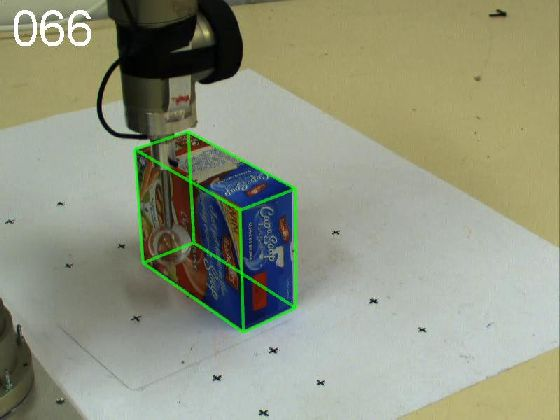
\includegraphics[width=\imgCXwid]{images/C1_2exp_87_1}
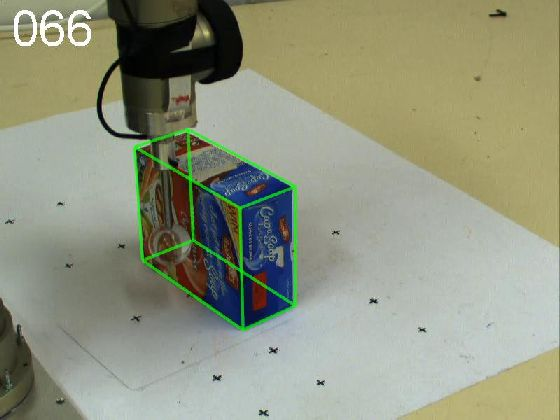
\includegraphics[width=\imgCXwid]{images/C1_1exp_87_1}
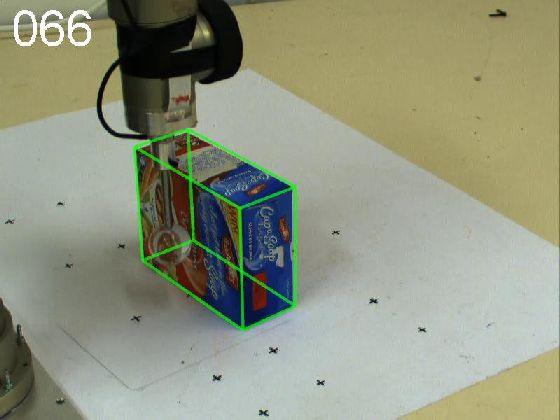
\includegraphics[width=\imgCXwid]{images/C1_LWPR1_87_1}
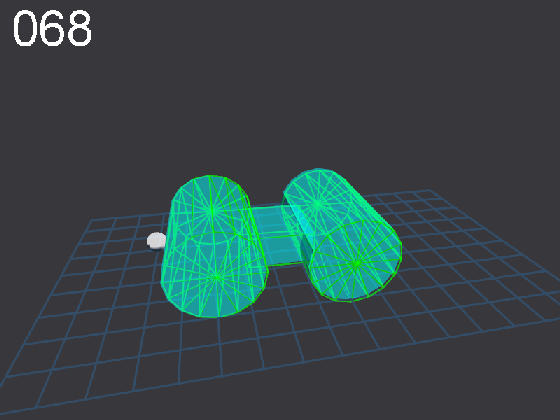
\includegraphics[width=\imgCXwid]{images/C5_1exp_6_1}
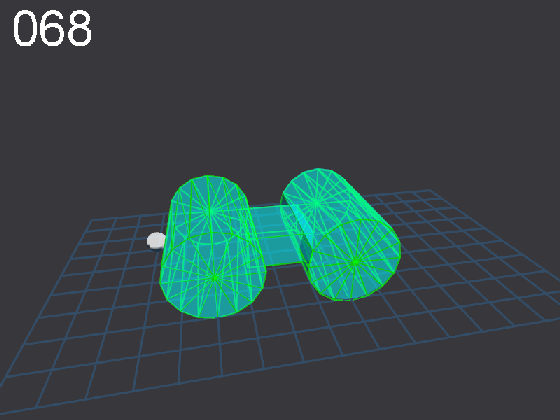
\includegraphics[width=\imgCXwid]{images/C5_2exp_6_1}
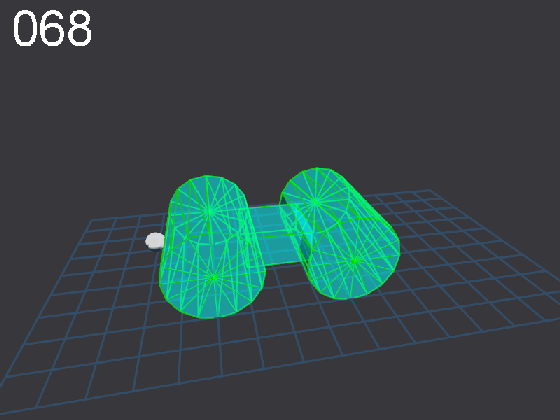
\includegraphics[width=\imgCXwid]{images/C5_3exp_6_1}
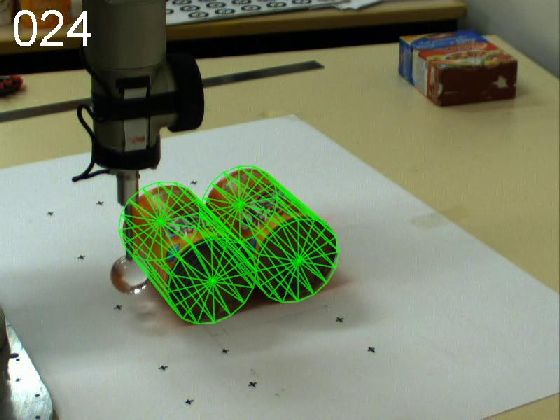
\includegraphics[width=\imgCXwid]{images/C2_3exp_75_1}
}
%\vspace{0.1cm}
\centerline{
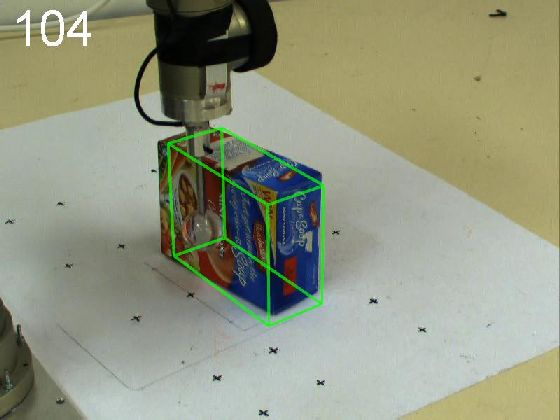
\includegraphics[width=\imgCXwid]{images/C1_2exp_87_2}
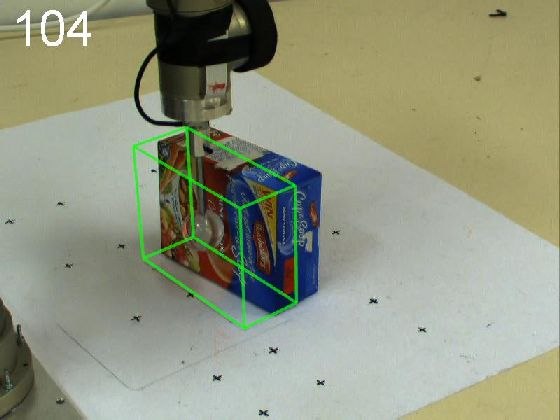
\includegraphics[width=\imgCXwid]{images/C1_1exp_87_2}
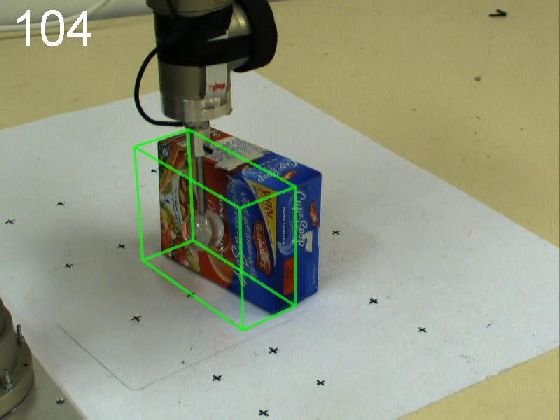
\includegraphics[width=\imgCXwid]{images/C1_LWPR1_87_2}
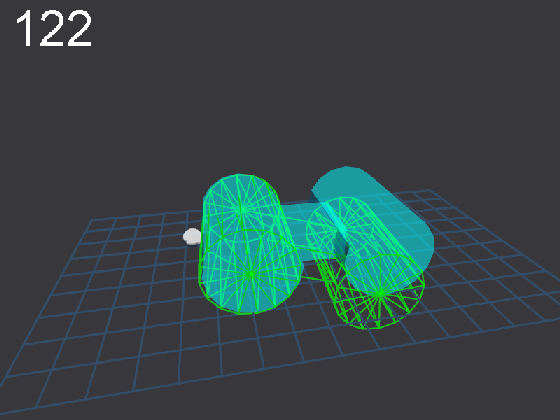
\includegraphics[width=\imgCXwid]{images/C5_1exp_6_2}
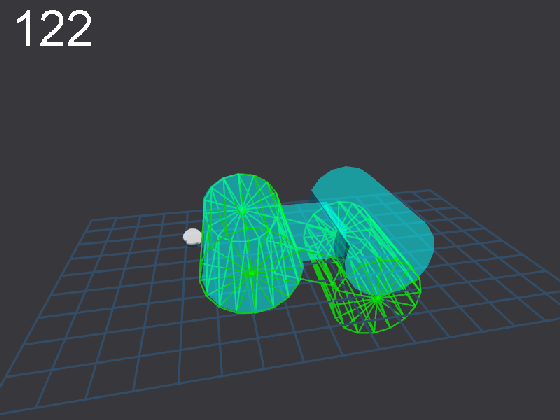
\includegraphics[width=\imgCXwid]{images/C5_2exp_6_2}
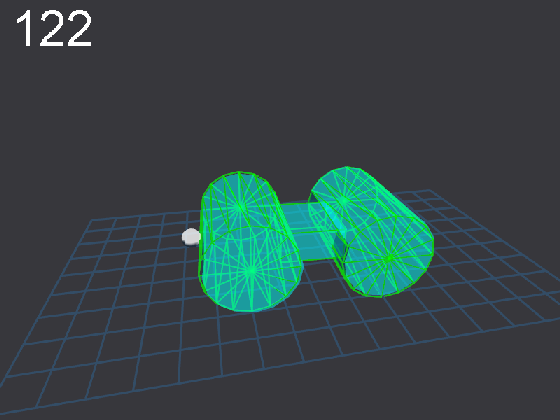
\includegraphics[width=\imgCXwid]{images/C5_3exp_6_2}
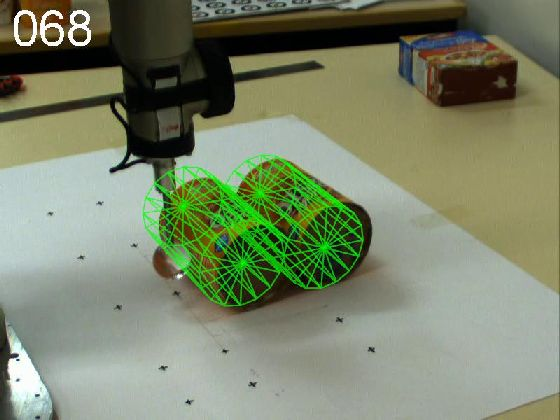
\includegraphics[width=\imgCXwid]{images/C2_3exp_75_2}
}
%\vspace{0.1cm}
\centerline{
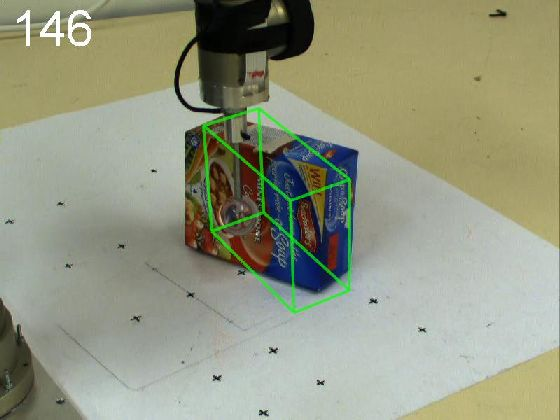
\includegraphics[width=\imgCXwid]{images/C1_2exp_87_3}
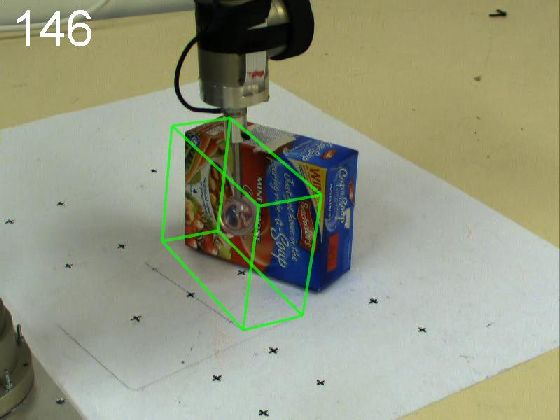
\includegraphics[width=\imgCXwid]{images/C1_1exp_87_3}
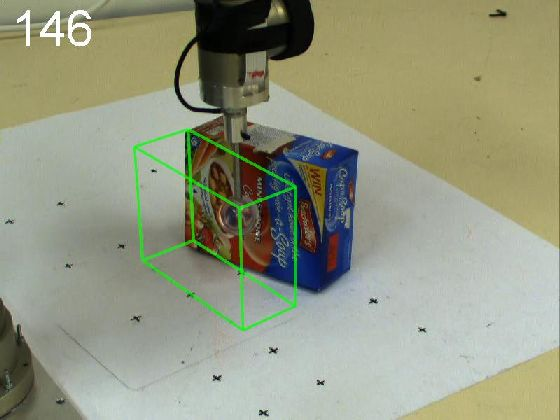
\includegraphics[width=\imgCXwid]{images/C1_LWPR1_87_3}
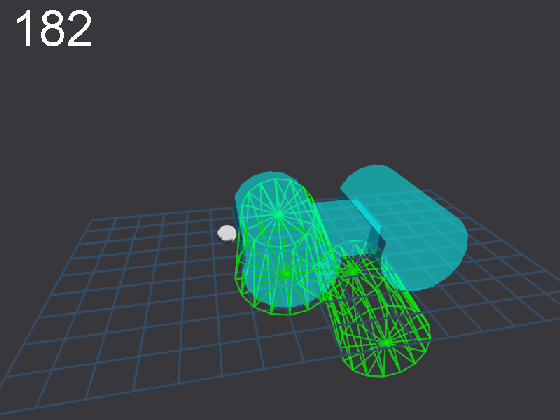
\includegraphics[width=\imgCXwid]{images/C5_1exp_6_3}
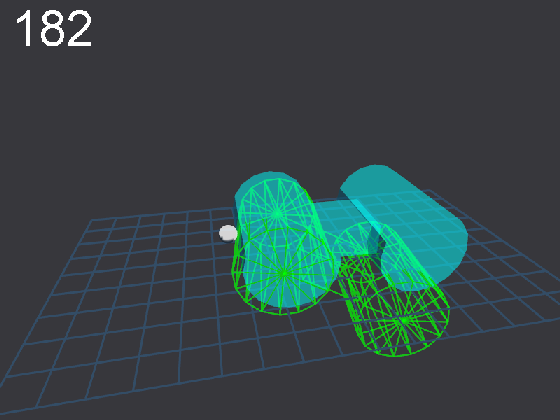
\includegraphics[width=\imgCXwid]{images/C5_2exp_6_3}
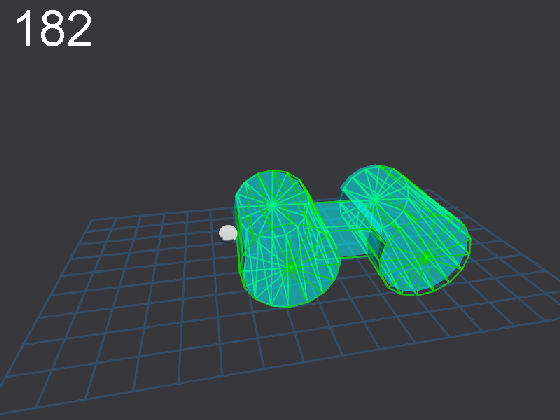
\includegraphics[width=\imgCXwid]{images/C5_3exp_6_3}
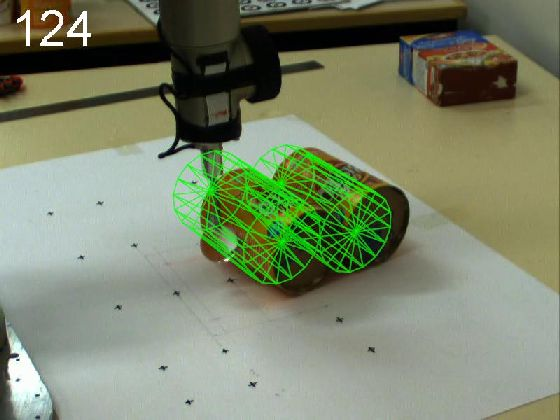
\includegraphics[width=\imgCXwid]{images/C2_3exp_75_3}
}
\centerline{
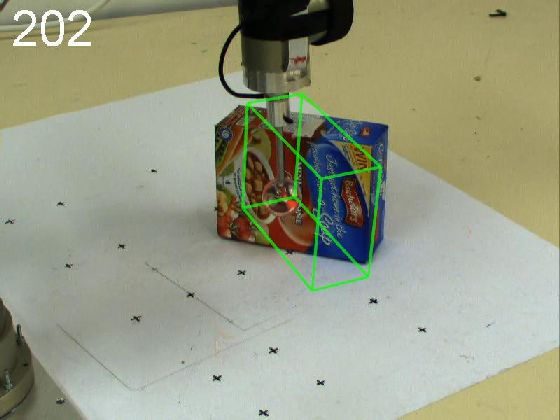
\includegraphics[width=\imgCXwid]{images/C1_2exp_87_4}
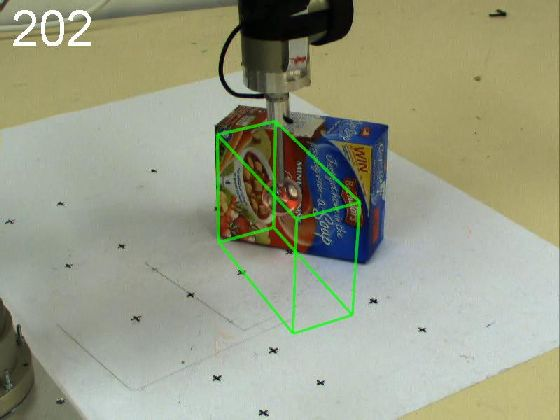
\includegraphics[width=\imgCXwid]{images/C1_1exp_87_4}
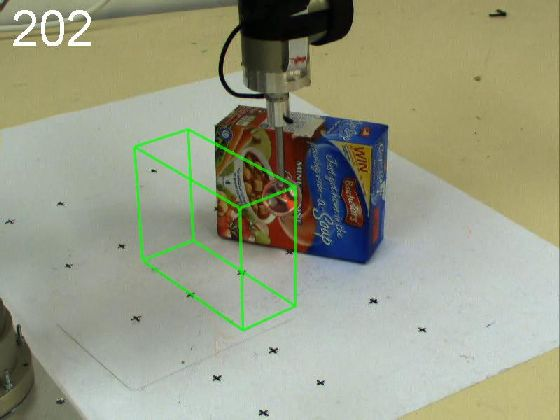
\includegraphics[width=\imgCXwid]{images/C1_LWPR1_87_4}
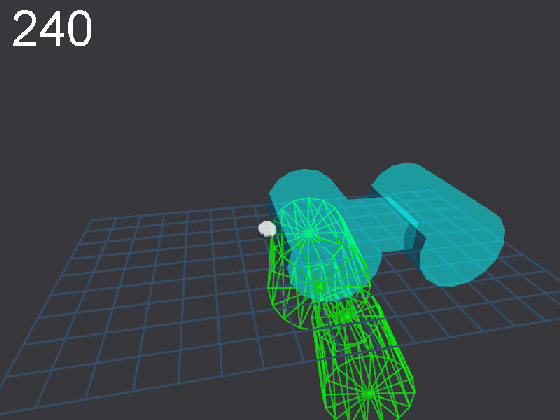
\includegraphics[width=\imgCXwid]{images/C5_1exp_6_4}
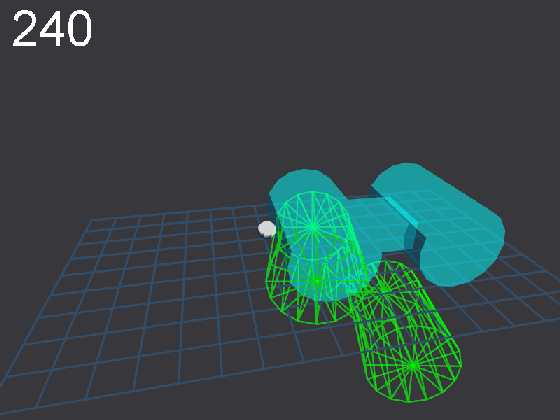
\includegraphics[width=\imgCXwid]{images/C5_2exp_6_4}
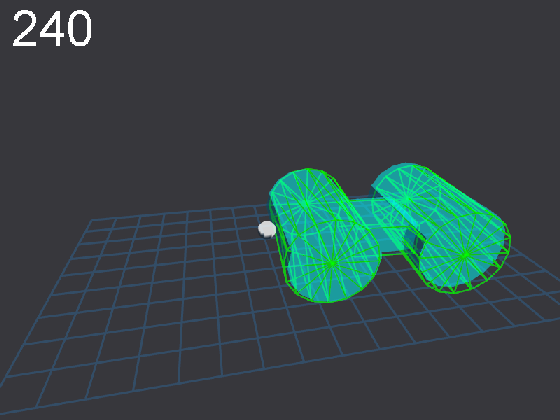
\includegraphics[width=\imgCXwid]{images/C5_3exp_6_4}
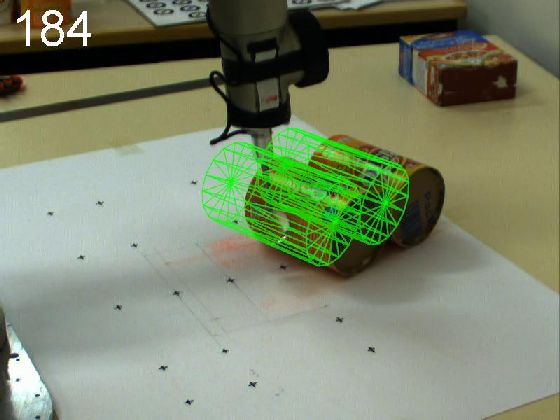
\includegraphics[width=\imgCXwid]{images/C2_3exp_75_4}
}
%\vspace{0.1cm}
\centerline{
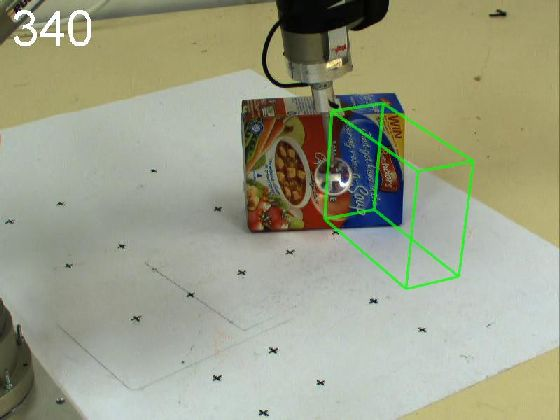
\includegraphics[width=\imgCXwid]{images/C1_2exp_87_5}
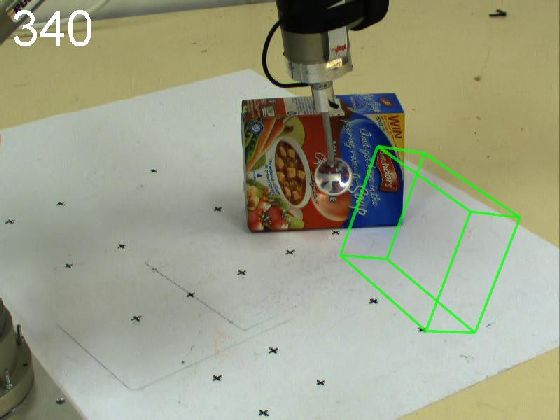
\includegraphics[width=\imgCXwid]{images/C1_1exp_87_5}
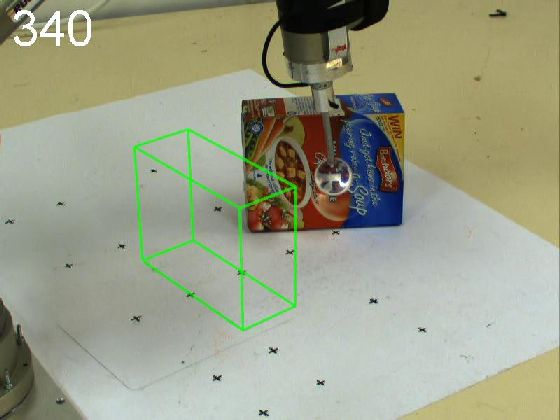
\includegraphics[width=\imgCXwid]{images/C1_LWPR1_87_5}
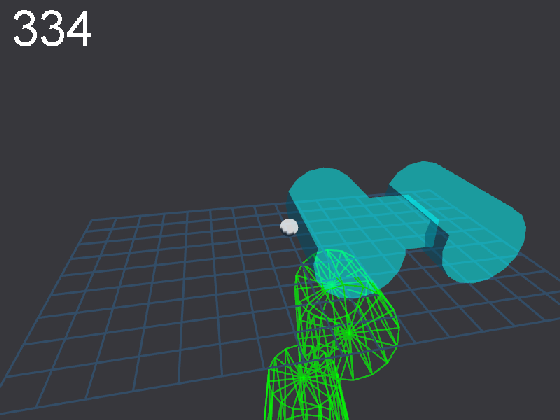
\includegraphics[width=\imgCXwid]{images/C5_1exp_6_5}
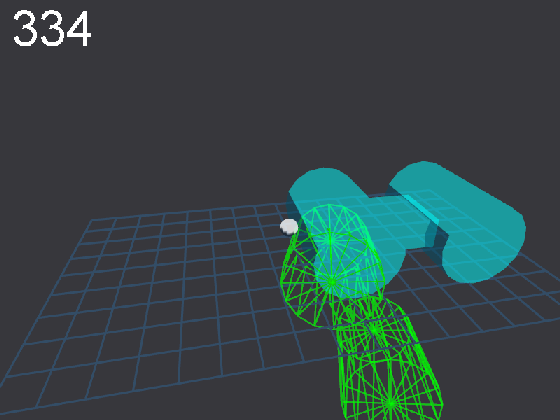
\includegraphics[width=\imgCXwid]{images/C5_2exp_6_5}
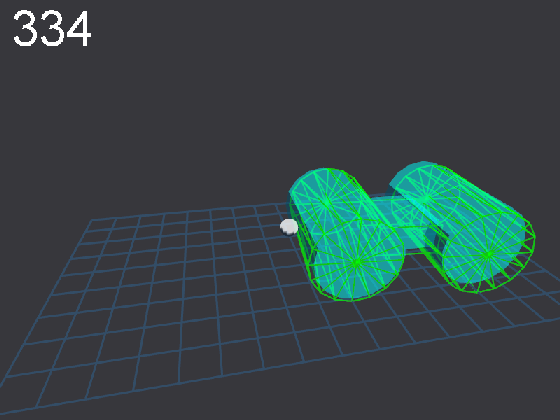
\includegraphics[width=\imgCXwid]{images/C5_3exp_6_5}
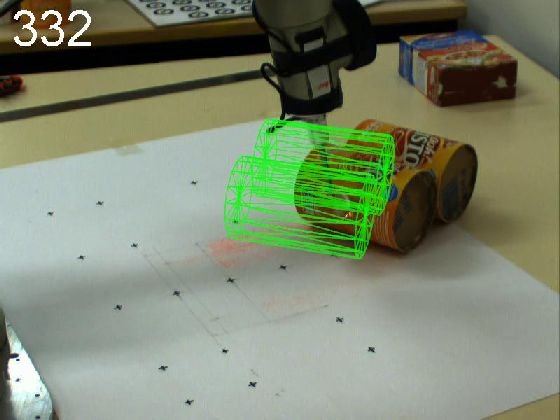
\includegraphics[width=\imgCXwid]{images/C2_3exp_75_5}
}

\caption {Experiment P3: Shape Transfer. Green outline shows predictions. Column~1: KDEF-GA/quat.
  Col~2: KDEF-G/quat. Col~3: LWPR-G for one trial.  Note that the
  KDEF-G/quat and LWPR-G methods predict that the robot finger moves
  into the box.  Col~4: KDEF-G/quat. Col~5: KDEF-GA/quat. Col~6:
  KDEF-GAE/quat. Col~7: KDEF-GAE/quat. The frame number is shown in
  the top left of each image.  }
\label{fig:ExperimentStransfer}
\end{figure*}

This paper has sought to establish a case for modular, machine learning approaches to metric prediction as a promising alternative to analytic modelling. Essentially machine learning plus modularisation allows us to predict accurately in the face of unobservable parameters. Unlike other learning approaches, ours provides precise predictions of rigid body motion over many steps, and can transfer predictions to novel actions and objects. This required exploiting the insight from analytic modelling that each contact must be modelled explicitly, and the structure of the learner should reflect the contact structure so as to to exploit this information. In summary combining insights from analytic and machine learning approaches is, we believe, the way forward.
